% =====================================================================
%  Figure captions for: Substitution-Tolerant Structural Correspondence
%
%  Every quantity quoted below is read from
%  validation/results/exp_correspondence.json and
%  validation/results/panel_data.json.  Minimum cuts are exact (maximum
%  flow); the only stochastic component anywhere is the rewiring control
%  of Figure 4, which seeds explicitly.
% =====================================================================

\begin{figure*}[!htbp]
    \centering
    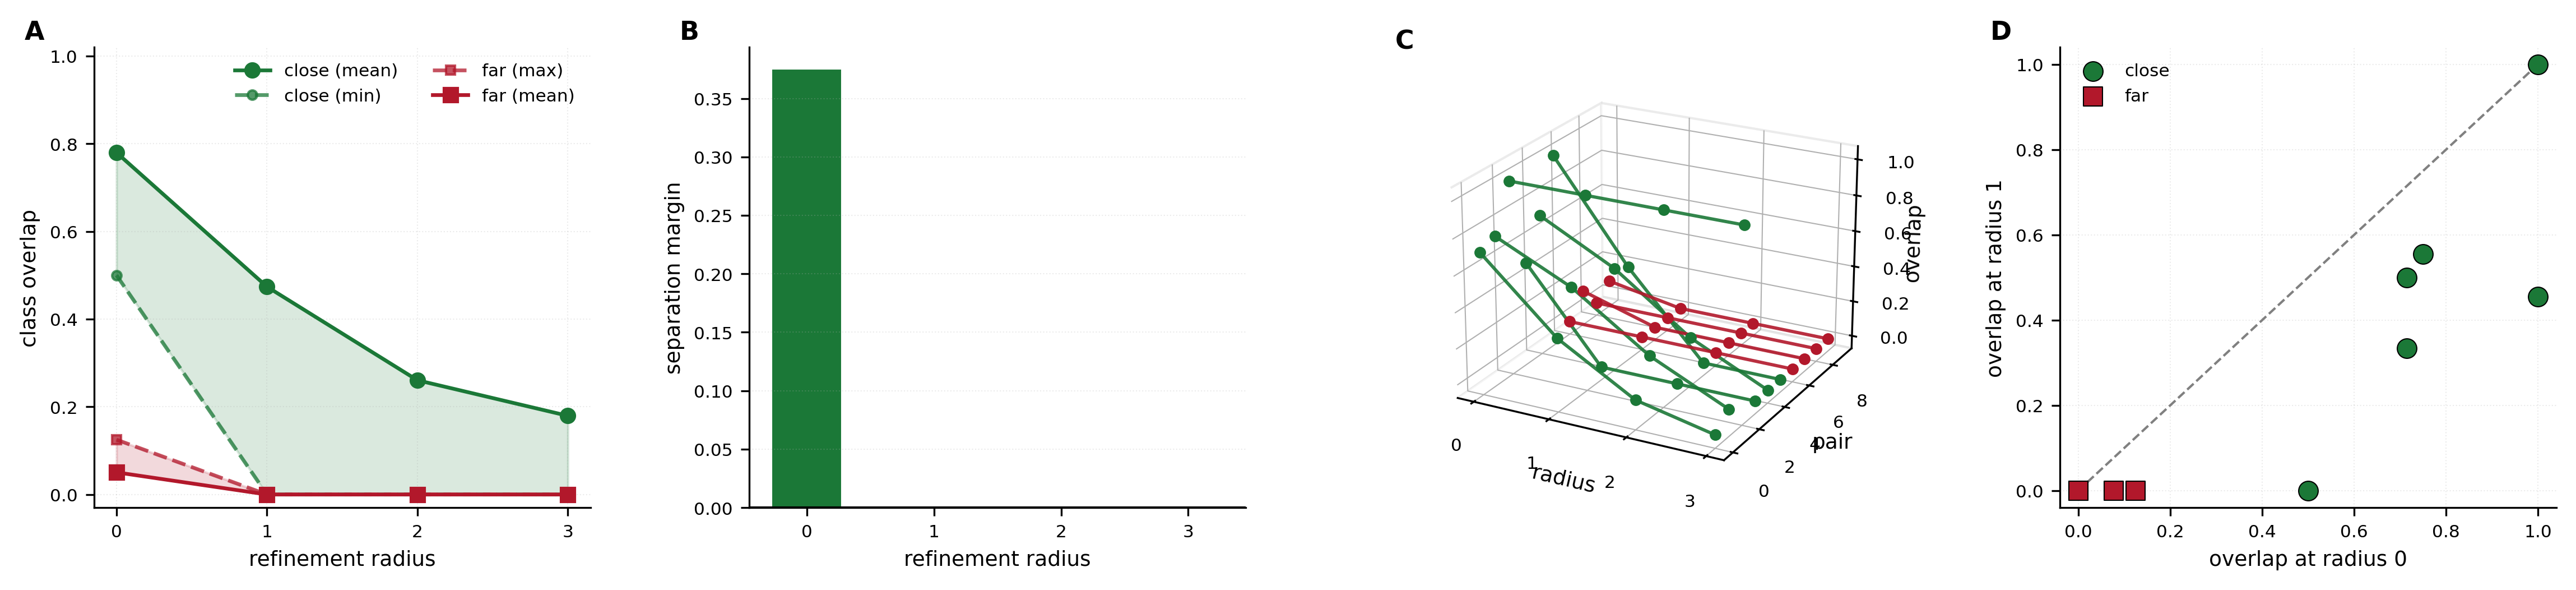
\includegraphics[width=\textwidth]{figures/panel_01_radius.png}
    \caption{\textbf{Tolerance is a resolution parameter, and the
    coarsest setting is the one that works: separation exists at radius
    $0$ and at no other radius.}
    Refinement radius indexes a family of labellings (\Cref{def:radius})
    that discriminate monotonically more (\Cref{lem:radius-order}), so a
    matcher's tolerance falls monotonically as radius rises. The
    prediction that radius $0$ would separate best was registered in the
    experiment source before the sweep was run.
    (\textbf{A})~Mean class overlap against radius for the
    \textsf{close} (green) and \textsf{far} (red) groups, with shaded
    bands running to the minimum \textsf{close} and maximum \textsf{far}
    value. The \textsf{close} mean falls $0.780 \to 0.474 \to 0.261 \to
    0.179$ across radii $0$--$3$, exactly the direction
    \Cref{prop:overlap-monotone} requires. The bands are disjoint only at
    radius $0$; from radius $1$ onward the minimum \textsf{close} value
    is $0.000$ and the groups touch.
    (\textbf{B})~The separation margin, minimum \textsf{close} minus
    maximum \textsf{far}: $+0.375$ at radius $0$ and exactly $0.000$ at
    radii $1$, $2$ and $3$. This is the paper's central measurement and
    it inverts the usual instinct --- making the matcher more
    discriminating does not improve it, it destroys it.
    (\textbf{C})~Every annotated pair traced across all four radii in
    three dimensions, \textsf{close} green and \textsf{far} red. The
    \textsf{close} traces descend toward the \textsf{far} floor
    individually, not merely on average, so the collapse in (\textbf{B})
    is not driven by a few pairs.
    (\textbf{D})~Overlap at radius $1$ against overlap at radius $0$ per
    pair, with the identity line. Every point lies on or below the
    diagonal --- no pair gains from refinement --- and one \textsf{close}
    pair falls from $0.500$ to $0.000$ in a single round. The mechanism is
    \Cref{rem:finer-worse}: at radius $1$ a label already encodes an
    atom's whole first neighbourhood, so one heteroatom substitution
    perturbs a neighbourhood's worth of labels at once.}
    \label{fig:radius}
\end{figure*}

\begin{figure*}[!htbp]
    \centering
    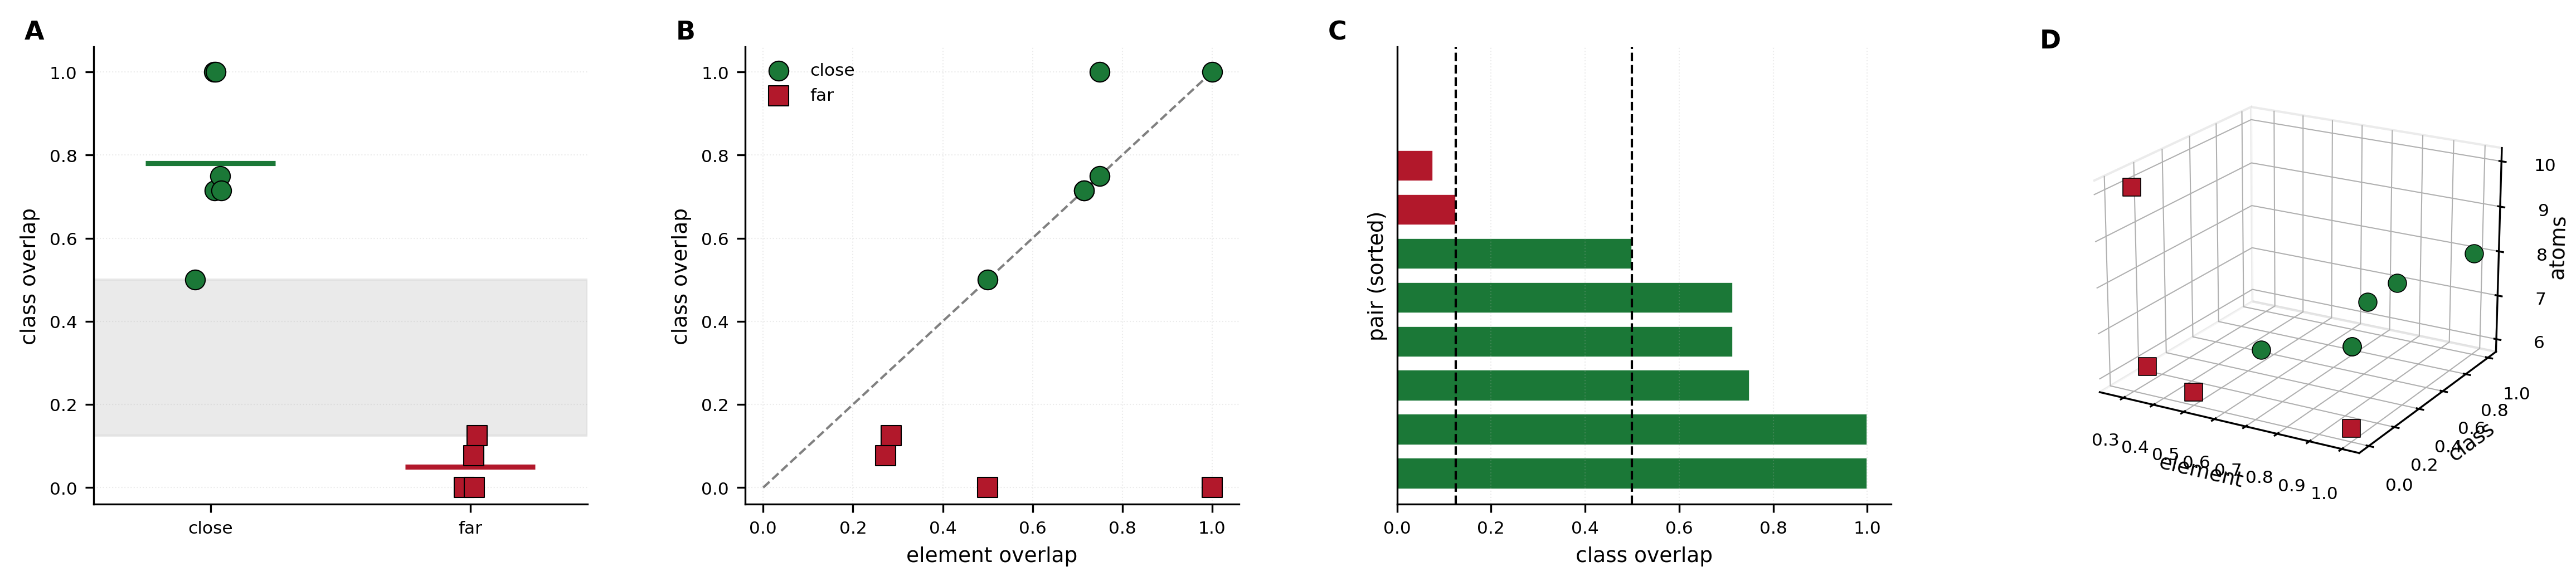
\includegraphics[width=\textwidth]{figures/panel_02_separation.png}
    \caption{\textbf{At the working radius the two annotated groups
    occupy disjoint ranges, and the pairs on which element identity and
    cut class most disagree are the informative ones.}
    The \textsf{close}/\textsf{far} annotations encode our reading of the
    medicinal-chemistry literature and were fixed before measurement;
    they are not derived from activity data (\Cref{sec:limits}).
    (\textbf{A})~Class overlap for the two groups with horizontal bars at
    the group means ($0.780$ and $0.050$). The shaded band spans the gap
    between the highest \textsf{far} value ($0.125$, ethanol/benzene) and
    the lowest \textsf{close} value ($0.500$, benzene/pyrazine); no pair
    lies inside it.
    (\textbf{B})~Class overlap against element overlap per pair with the
    identity line. The two \textsf{far} points on the floor are the
    substantive cases: benzene/cyclohexane at element $1.000$ and class
    $0.000$, and propane/pyridine at element $0.500$ and class $0.000$.
    Benzene and cyclohexane are compositionally identical --- six carbons
    each --- so an element-keyed comparison cannot separate them at all,
    while the cut class finds no shared structural role whatever. This is
    the clearest single demonstration that the invariant is not a
    relabelling of element identity.
    (\textbf{C})~All ten pairs sorted by class overlap, with the two
    dashed lines marking the boundaries of the empty band. Four
    \textsf{close} pairs share their element overlap exactly with their
    class overlap ($0.714$, $0.714$, $0.750$, $0.500$), so on those the
    tolerance is not doing work; the effect is concentrated in the pairs
    where the two differ.
    (\textbf{D})~Element overlap, class overlap and the size of the larger
    structure in three dimensions. The green and red point sets separate
    along the class axis at every size, so the separation in (\textbf{A})
    is not an artefact of the \textsf{far} pairs happening to be larger or
    smaller than the \textsf{close} ones.}
    \label{fig:separation}
\end{figure*}

\begin{figure*}[!htbp]
    \centering
    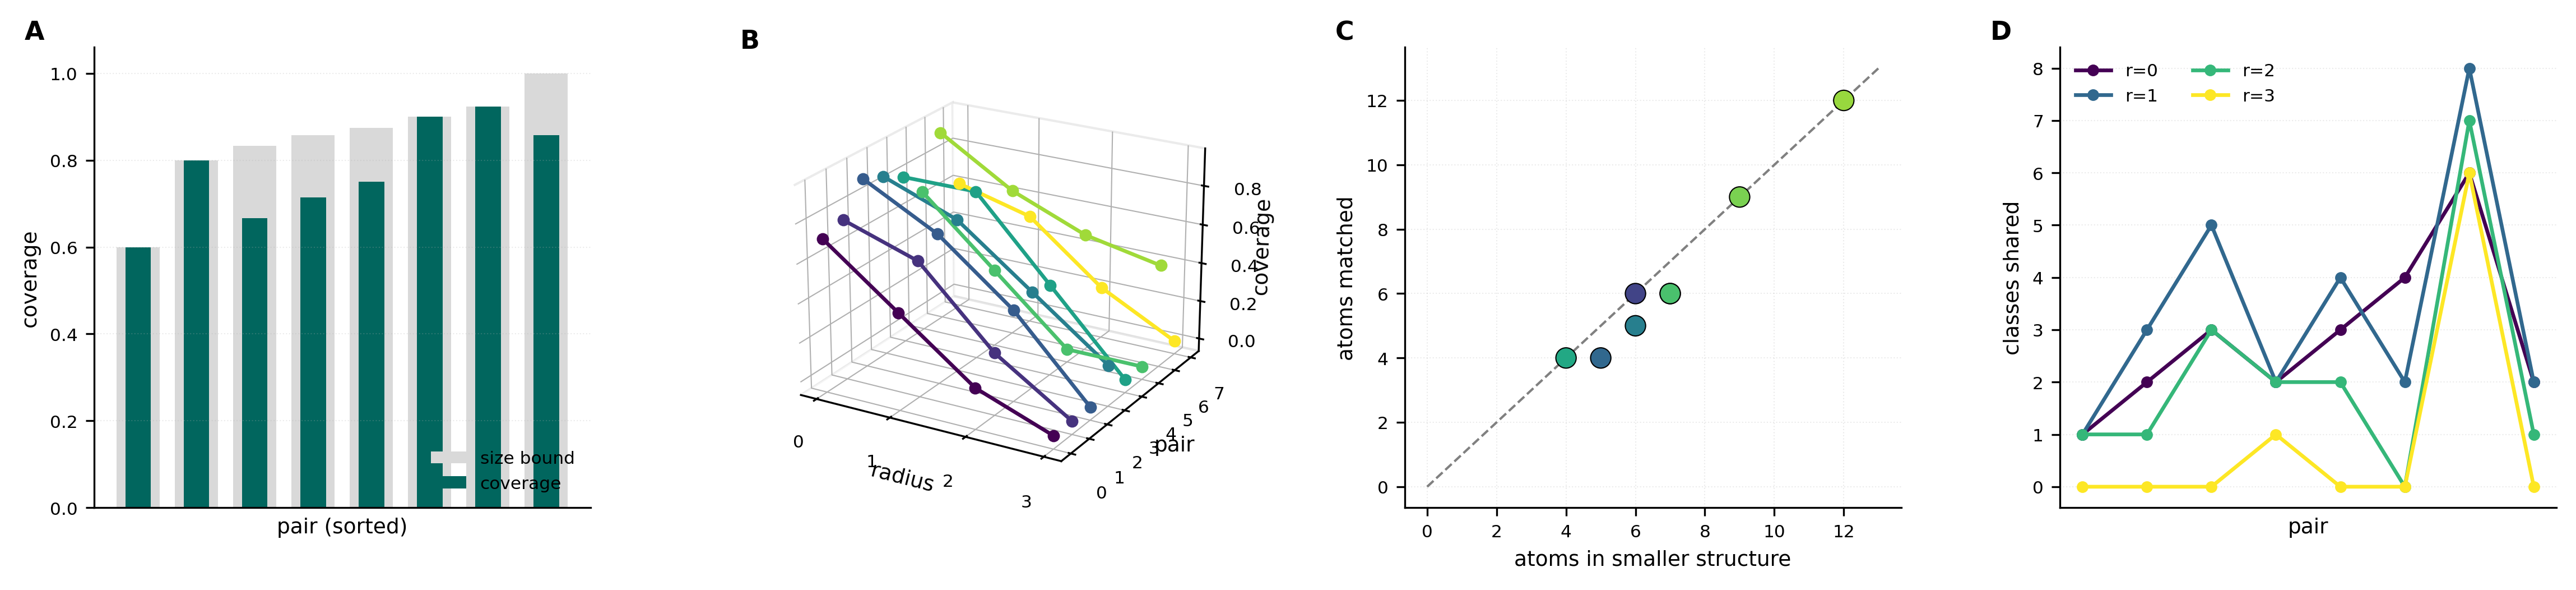
\includegraphics[width=\textwidth]{figures/panel_03_correspondence.png}
    \caption{\textbf{Correspondence on one-position matched pairs, and
    the same radius erosion seen in the correspondence itself rather than
    in the overlap.}
    Correspondence is computed without search (\Cref{prop:cost}); it is
    not a maximum common substructure and carries no connectivity
    guarantee (\Cref{sec:limits}).
    (\textbf{A})~Coverage (teal) against the size bound
    $\min(n_1,n_2)/\max(n_1,n_2)$ (grey) per pair, sorted. Mean coverage
    is $0.776$ with median $0.775$ and minimum $0.600$, and $3$ of the $8$
    pairs sit exactly at their ceiling --- every atom of the smaller
    structure found a correspondent. Raw coverage therefore understates
    match quality for pairs of unequal size, and normalising by the bound
    is a correction we have not applied.
    (\textbf{B})~Coverage against radius for each matched pair in three
    dimensions. Mean coverage falls $0.776 \to 0.599 \to 0.295 \to 0.076$
    across radii $0$--$3$: the same monotone erosion \Cref{fig:radius}
    shows for overlap, now visible in the number of atoms actually paired.
    By radius $3$ the matcher pairs almost nothing.
    (\textbf{C})~Atoms matched against the atom count of the smaller
    structure, with the identity line and colour by coverage. Points on
    the line are the three pairs at their size bound; the vertical drop
    for the others is the number of atoms the substitution displaced far
    enough in cut-key terms to break the correspondence.
    (\textbf{D})~Classes shared between the two structures of each pair at
    each radius. The curves fall together rather than crossing, so no pair
    is anomalously robust to refinement --- the erosion is a property of
    the labelling, not of particular molecules.}
    \label{fig:corr}
\end{figure*}

\begin{figure*}[!htbp]
    \centering
    
\includegraphics[width=\textwidth]{figures/panel_04_control.png}
    \caption{\textbf{The rewiring control destroys the separation, and the
    cross-element gain --- the effect the method is motivated by --- is
    real but small.}
    An earlier control permuted class labels within each structure; that
    is a no-op on a multiset and reported a margin identical to the true
    one, so it could not fail and certified nothing (\Cref{sec:errors}).
    The control below rewires instead.
    (\textbf{A})~Separation margin for the true structures ($+0.375$) and
    after rewiring the second structure of each pair at random while
    holding atom composition and edge count fixed ($-0.069$, mean over
    $20$ seeds per pair). The margin does not merely shrink; it reverses
    sign, so the two groups overlap under the control.
    (\textbf{B})~Group means before and after rewiring. The
    \textsf{close} mean collapses $0.780 \to 0.063$ while the \textsf{far}
    mean barely moves, $0.050 \to 0.041$. The asymmetry is the point:
    rewiring has nothing to destroy in pairs that never shared structure,
    and everything to destroy in pairs that did.
    (\textbf{C})~Margin over radius under both conditions in three
    dimensions. The true margin exists at radius $0$ and nowhere else; the
    rewired margin is negative at every radius. The two surfaces together
    show that the effect requires both the coarse radius and the true
    connectivity --- neither alone produces it.
    (\textbf{D})~Pairings admitted per \textsf{close} pair, split into
    same-element (blue) and cross-element (orange). Cross-element pairings
    are exactly what an element-keyed matcher cannot make, and they total
    $4$ across the six pairs, occurring in $3$ of them; mean coverage is
    $0.865$ with them and $0.776$ without. This is the paper's weakest
    measurement and we report it as such: the gain concentrates where the
    substituted atom is peripheral and vanishes where the heteroatom sits
    inside a ring, a pattern six pairs cannot establish.}
    \label{fig:rewire}
\end{figure*}

\begin{figure*}[!htbp]
    \centering
    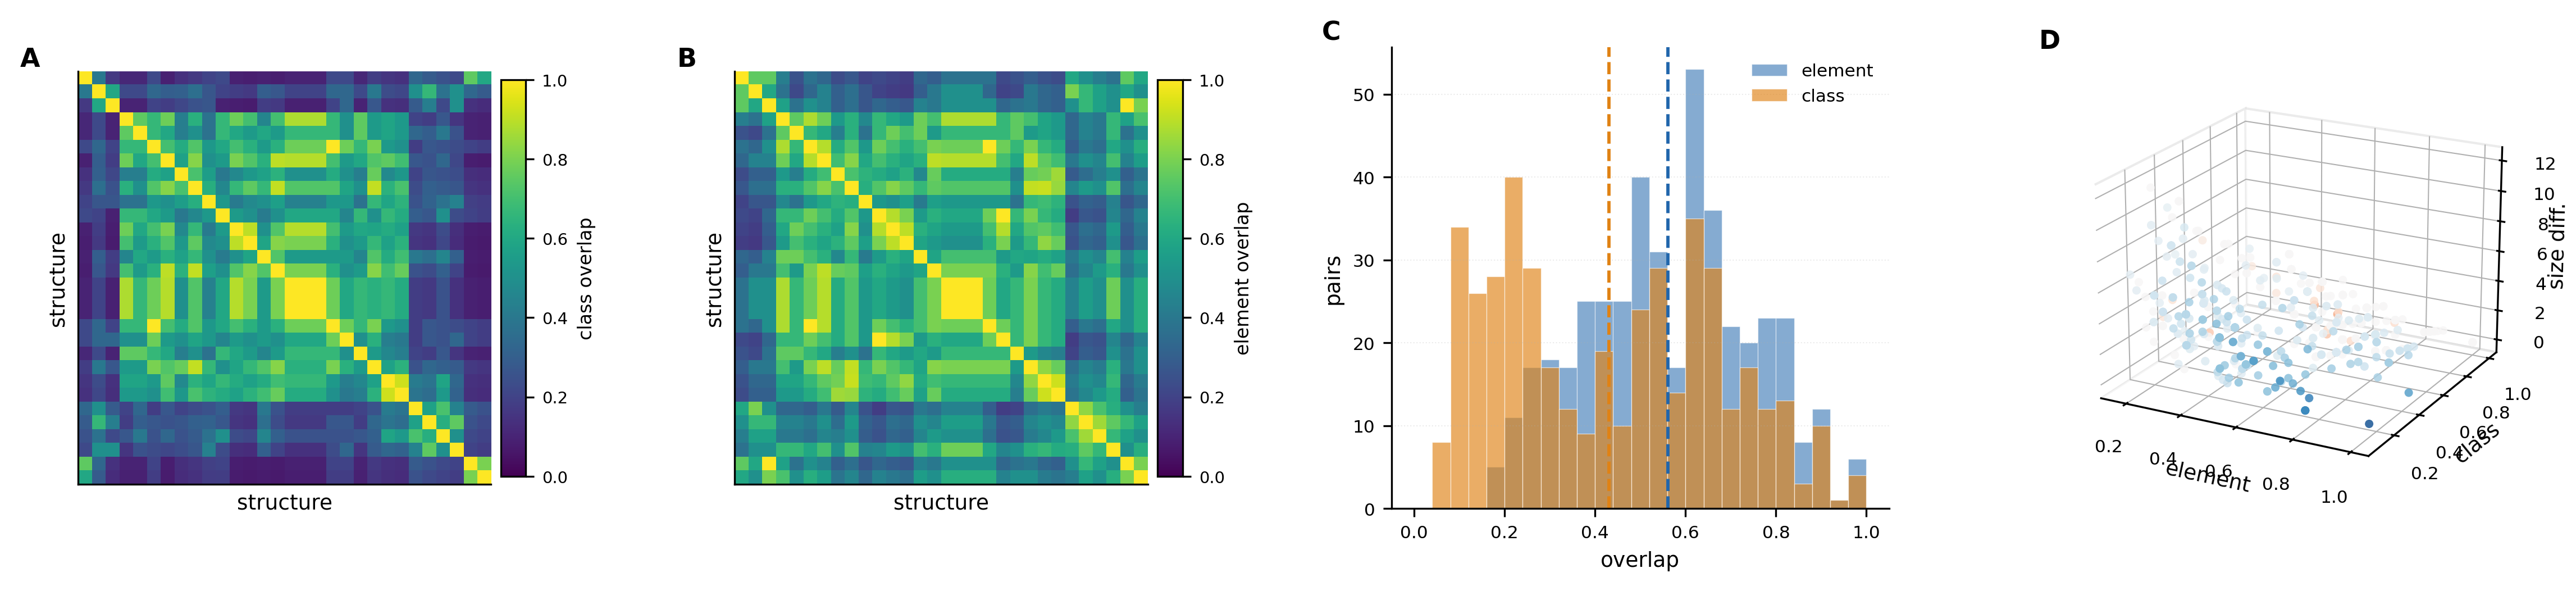
\includegraphics[width=\textwidth]{figures/panel_05_matrix.png}
    \caption{\textbf{Over $435$ pairs of the drug-like corpus, class
    overlap and element overlap have visibly different structure and are
    not proxies for one another.}
    All values are at radius $0$; the corpus is thirty small organic
    structures and no reference annotation is asserted for these pairs,
    so the panel is descriptive rather than a test.
    (\textbf{A})~Class-overlap matrix for all $\binom{30}{2}$ pairs,
    structures in corpus order.
    (\textbf{B})~Element-overlap matrix for the same pairs on the same
    colour scale. The block structure differs visibly from (\textbf{A}):
    regions bright in one are dim in the other, which is the matrix form
    of the benzene/cyclohexane observation in \Cref{fig:separation}.
    (\textbf{C})~Distributions of the two overlaps with their means
    marked. Class overlap is shifted left --- mean $0.430$, median
    $0.429$ --- against element overlap at mean $0.561$, median $0.571$.
    Agreeing on composition is easier than agreeing on structural role,
    so the class criterion is the stricter of the two on a random pair;
    it is the more permissive one only on pairs that are structurally
    analogous, which is the behaviour the method is for.
    (\textbf{D})~Element overlap, class overlap and absolute size
    difference in three dimensions, coloured by class minus element
    overlap. Of the $435$ pairs, $257$ have class overlap below element
    overlap and $23$ above; no pair has zero class overlap. The points
    furthest from the diagonal plane are those on which the two criteria
    most disagree, and they are distributed across all size differences
    rather than concentrated among pairs of very unequal size.}
    \label{fig:matrix}
\end{figure*}
